% Corresponding source for the AGPL-derived gallery PNG.
\RequirePackage{fix-cm}
\documentclass{article}
\usepackage[paperwidth=268.828mm,paperheight=174.57mm,margin=5mm]{geometry}
\usepackage{graphicx}
\usepackage{fontspec}
\usepackage{xeCJK}
\IfFontExistsTF{PingFang SC}{\setCJKmainfont{PingFang SC}}{\IfFontExistsTF{Noto Sans CJK SC}{\setCJKmainfont{Noto Sans CJK SC}}{\IfFontExistsTF{Heiti SC}{\setCJKmainfont{Heiti SC}}{\setCJKmainfont{FandolHei-Regular}}}}
\usepackage{tikz}
\usetikzlibrary{arrows.meta,calc,positioning,fit,backgrounds,shapes.geometric}
\pagestyle{empty}
\newcommand{\CaptureTikZPositions}{}
% Edit shared fonts, component sizes, gaps, borders and arrows here.
\definecolor{ink0}{HTML}{000000}
\definecolor{ink1}{HTML}{888888}
\definecolor{ink2}{HTML}{555555}
\definecolor{ink3}{HTML}{777777}
\definecolor{ink4}{HTML}{FFFFFF}
\definecolor{ink5}{HTML}{F6D7D7}
\definecolor{ink6}{HTML}{FCE9D5}
\definecolor{ink7}{HTML}{D7D5F6}
\definecolor{ink8}{HTML}{DAEFDA}
\definecolor{ink9}{HTML}{E5E5EF}
\definecolor{ink10}{HTML}{E5EBE5}
\definecolor{ink11}{HTML}{CCCBDD}
\definecolor{ink12}{HTML}{E3F2FF}
\definecolor{ink13}{HTML}{E5F5E5}
\definecolor{ink14}{HTML}{FFF2E5}
\newcommand{\FontA}{\fontsize{8.67188}{10.4062}\selectfont\rmfamily\mdseries\color{ink0}}
\newcommand{\FontB}{\fontsize{7.58789}{9.10547}\selectfont\rmfamily\mdseries\color{ink0}}
\newcommand{\FontC}{\fontsize{8.67188}{10.4062}\selectfont\rmfamily\bfseries\color{ink0}}
\newcommand{\FontD}{\fontsize{8.67188}{10.4062}\selectfont\rmfamily\mdseries\color{ink1}}
\newcommand{\FontE}{\fontsize{7.5}{9}\selectfont\rmfamily\mdseries\color{ink0}}
\newcommand{\WidthA}{91.6406mm}
\newcommand{\HeightA}{37.9688mm}
\newcommand{\WidthB}{46.0547mm}
\newcommand{\HeightB}{51.7969mm}
\newcommand{\WidthC}{43.3594mm}
\newcommand{\HeightC}{82.3828mm}
\newcommand{\WidthD}{32.5781mm}
\newcommand{\HeightD}{43.3594mm}
\newcommand{\WidthE}{32.5781mm}
\newcommand{\HeightE}{67.7344mm}
\newcommand{\WidthF}{59.7656mm}
\newcommand{\HeightF}{70.5469mm}
\newcommand{\WidthG}{40.1953mm}
\newcommand{\HeightG}{65.1562mm}
\newcommand{\WidthH}{17.5781mm}
\newcommand{\HeightH}{4.10156mm}
\newcommand{\WidthI}{14.7656mm}
\newcommand{\HeightI}{4.10156mm}
\newcommand{\WidthJ}{51.5625mm}
\newcommand{\HeightJ}{3.75mm}
\newcommand{\WidthK}{21.6797mm}
\newcommand{\HeightK}{8.67188mm}
\newcommand{\WidthL}{3.51562mm}
\newcommand{\HeightL}{3.51562mm}
\newcommand{\WidthM}{21.6797mm}
\newcommand{\HeightM}{4.33594mm}
\newcommand{\WidthN}{21.6797mm}
\newcommand{\HeightN}{11.9531mm}
\newcommand{\WidthO}{15.2344mm}
\newcommand{\HeightO}{4.6875mm}
\newcommand{\WidthP}{24.6094mm}
\newcommand{\HeightP}{8.90625mm}
\newcommand{\WidthQ}{25.1953mm}
\newcommand{\HeightQ}{7.61719mm}
\newcommand{\WidthR}{15.8203mm}
\newcommand{\HeightR}{7.03125mm}
\newcommand{\WidthS}{14.5312mm}
\newcommand{\HeightS}{7.03125mm}
\newcommand{\WidthT}{6.5625mm}
\newcommand{\HeightT}{6.5625mm}
\newcommand{\WidthU}{5.85938mm}
\newcommand{\HeightU}{5.03906mm}
\newcommand{\WidthV}{7.03125mm}
\newcommand{\HeightV}{5.03906mm}
\newcommand{\WidthW}{21.0938mm}
\newcommand{\HeightW}{8.20312mm}
\newcommand{\WidthX}{21.6797mm}
\newcommand{\HeightX}{8.20312mm}
\newcommand{\WidthY}{11.9531mm}
\newcommand{\HeightY}{4.33594mm}
\newcommand{\WidthZ}{6.09375mm}
\newcommand{\HeightZ}{4.57031mm}
\newcommand{\WidthAA}{46.6406mm}
\newcommand{\HeightAA}{8.67188mm}
\newcommand{\WidthAB}{32.4609mm}
\newcommand{\HeightAB}{8.67188mm}
\newcommand{\WidthAC}{19.4531mm}
\newcommand{\HeightAC}{4.33594mm}
\newcommand{\WidthAD}{4.6875mm}
\newcommand{\HeightAD}{4.6875mm}
\newcommand{\WidthAE}{11.9531mm}
\newcommand{\HeightAE}{10.7812mm}
\newcommand{\WidthAF}{7.03125mm}
\newcommand{\HeightAF}{16.9922mm}

% Local geometry: x right, y down; one macro call per semantic component.
\newcommand{\FeatureStack}[8]{%
\begin{scope}[shift={(#1.north west)},x=1mm,y=-1mm]
\pgfmathtruncatemacro{\lastface}{#4-1}
\foreach \i in {0,...,\lastface}{%
\ifodd\i\def\facecolor{#8}\else\def\facecolor{#7}\fi
\fill[\facecolor] ({\i*#5},{\i*#6}) rectangle ++(#2,#3);
}
\end{scope}}
\newcommand{\TensorSlab}[5]{%
\begin{scope}[shift={(#1.north west)},x=1mm,y=-1mm]
\fill[#5] (0,0)--(#2,0)--({#2+#4},#3)--(#4,#3)--cycle;
\end{scope}}

\tikzset{
border-plain/.style={draw=ink0,line width=0.35pt,solid,line cap=round,line join=round},
edge-plain/.style={border-plain,-},
border-flow/.style={draw=ink0,line width=0.35pt,solid,line cap=round,line join=round},
edge-flow/.style={border-flow,->},
border-dots/.style={draw=ink2,line width=0.3pt,dotted,line cap=round,line join=round},
edge-dots/.style={border-dots,-},
border-dash/.style={draw=ink0,line width=0.35pt,dashed,line cap=round,line join=round},
edge-dash/.style={border-dash,-},
border-zoom/.style={draw=ink3,line width=0.35pt,dotted,line cap=round,line join=round},
edge-zoom/.style={border-zoom,-},
node-label/.style={border-plain,fill=ink4,rectangle,draw=none,fill=none,align=center,inner sep=0.05mm,outer sep=0pt,opacity=1,fill opacity=1,font=\FontA},
node-heading/.style={border-plain,fill=ink4,rectangle,draw=none,fill=none,align=center,inner sep=0.05mm,outer sep=0pt,opacity=1,fill opacity=1,font=\FontC},
node-zoomlabel/.style={border-plain,fill=ink4,rectangle,draw=none,fill=none,align=center,inner sep=0.05mm,outer sep=0pt,opacity=1,fill opacity=1,font=\FontD},
node-embedding/.style={border-plain,fill=ink5,rectangle,rounded corners=0.4mm,align=center,inner sep=0.05mm,outer sep=0pt,opacity=1,fill opacity=1,font=\FontA},
node-attention/.style={border-plain,fill=ink6,rectangle,rounded corners=0.4mm,align=center,inner sep=0.05mm,outer sep=0pt,opacity=1,fill opacity=1,font=\FontA},
node-feed/.style={border-plain,fill=ink7,rectangle,rounded corners=0.4mm,align=center,inner sep=0.05mm,outer sep=0pt,opacity=1,fill opacity=1,font=\FontA},
node-norm/.style={border-plain,fill=ink8,rectangle,rounded corners=0.4mm,align=center,inner sep=0.05mm,outer sep=0pt,opacity=1,fill opacity=1,font=\FontA},
node-linear/.style={border-plain,fill=ink9,rectangle,rounded corners=0.4mm,align=center,inner sep=0.05mm,outer sep=0pt,opacity=1,fill opacity=1,font=\FontA},
node-softmax/.style={border-plain,fill=ink10,rectangle,rounded corners=0.4mm,align=center,inner sep=0.05mm,outer sep=0pt,opacity=1,fill opacity=1,font=\FontA},
node-scaled/.style={border-plain,fill=ink11,rectangle,rounded corners=0.4mm,align=center,inner sep=0.05mm,outer sep=0pt,opacity=1,fill opacity=1,font=\FontA},
node-encoder/.style={border-dots,fill=ink12,rectangle,align=center,inner sep=0.05mm,outer sep=0pt,opacity=1,fill opacity=1,font=\FontA},
node-decoder/.style={border-dots,fill=ink13,rectangle,align=center,inner sep=0.05mm,outer sep=0pt,opacity=1,fill opacity=1,font=\FontA},
node-preprocessing/.style={border-dots,fill=ink14,rectangle,align=center,inner sep=0.05mm,outer sep=0pt,opacity=1,fill opacity=1,font=\FontA},
node-repeat/.style={border-dash,fill=ink4,rectangle,align=center,inner sep=0.05mm,outer sep=0pt,opacity=1,fill opacity=0,font=\FontA},
node-detail/.style={border-dots,fill=ink4,rectangle,align=center,inner sep=0.05mm,outer sep=0pt,opacity=1,fill opacity=0,font=\FontA},
node-headlabel/.style={border-dots,fill=ink4,rectangle,align=center,inner sep=0.05mm,outer sep=0pt,opacity=1,fill opacity=1,font=\FontA},
node-sum/.style={border-plain,fill=ink14,ellipse,align=center,inner sep=0.05mm,outer sep=0pt,opacity=1,fill opacity=1,font=\FontE},
node-ghostlinear/.style={border-plain,fill=ink9,rectangle,rounded corners=0.4mm,align=center,inner sep=0.05mm,outer sep=0pt,opacity=0.5,fill opacity=0.5,font=\FontA},
node-ghostscaled/.style={border-plain,fill=ink11,rectangle,rounded corners=0.4mm,align=center,inner sep=0.05mm,outer sep=0pt,opacity=0.5,fill opacity=0.5,font=\FontA},
node-position-label/.style={border-plain,fill=ink4,rectangle,draw=none,fill=none,align=center,inner sep=0.05mm,outer sep=0pt,opacity=1,fill opacity=1,font=\FontB}
}

\begin{document}
\noindent% Editable native TikZ. Positive scene y points down.
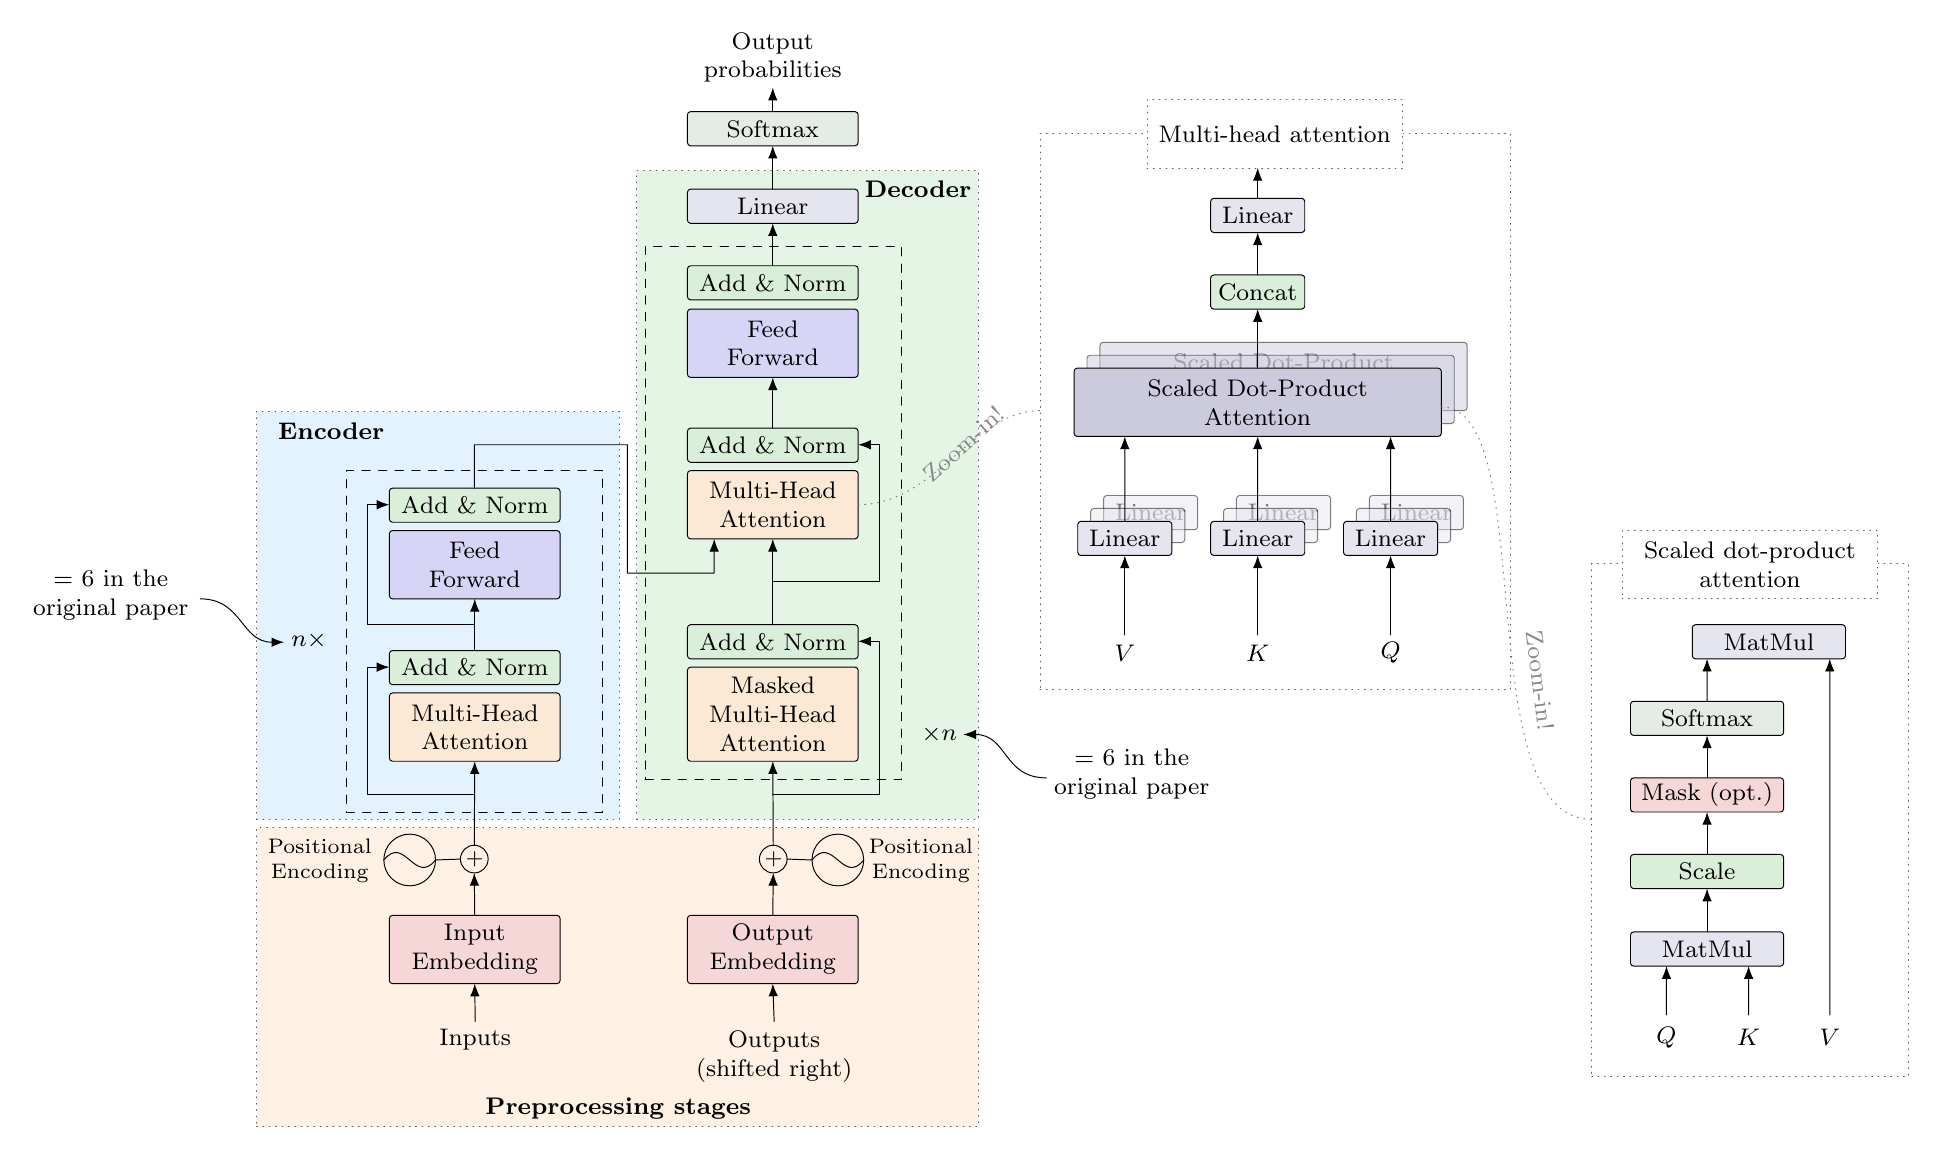
\begin{tikzpicture}[>=Latex]
\node[node-preprocessing,minimum width=\WidthA,minimum height=\HeightA,text width=\dimexpr\WidthA*1000/1000-0.1mm\relax] (pre) at (74.8828mm,-120.586mm) {};
\node[node-encoder,minimum width=\WidthB,minimum height=\HeightB,text width=\dimexpr\WidthB*1000/1000-0.1mm\relax] (enc) at ($(pre)+(-22.793mm,45.9375mm)$) {};
\node[node-decoder,minimum width=\WidthC,minimum height=\HeightC,text width=\dimexpr\WidthC*1000/1000-0.1mm\relax] (dec) at ($(pre)+(24.1406mm,61.2305mm)$) {};
\node[node-repeat,minimum width=\WidthD,minimum height=\HeightD,text width=\dimexpr\WidthD*1000/1000-0.1mm\relax] (enc-repeat) at ($(enc)+(4.62891mm,-3.28125mm)$) {};
\node[node-repeat,minimum width=\WidthE,minimum height=\HeightE,text width=\dimexpr\WidthE*1000/1000-0.1mm\relax] (dec-repeat) at ($(dec)+(-4.33594mm,-2.28516mm)$) {};
\node[node-detail,minimum width=\WidthF,minimum height=\HeightF,text width=\dimexpr\WidthF*1000/1000-0.1mm\relax] (detail-heads) at ($(dec)+(59.4141mm,10.6055mm)$) {};
\node[node-detail,minimum width=\WidthG,minimum height=\HeightG,text width=\dimexpr\WidthG*1000/1000-0.1mm\relax] (detail-dot) at ($(detail-heads)+(60.293mm,-51.9141mm)$) {};
\node[node-heading,minimum width=\WidthH,minimum height=\HeightH,text width=\dimexpr\WidthH*1000/1000-0.1mm\relax] (enc-title) at ($(enc)+(-13.5352mm,23.3789mm)$) {Encoder};
\node[node-heading,minimum width=\WidthI,minimum height=\HeightI,text width=\dimexpr\WidthI*1000/1000-0.1mm\relax] (dec-title) at ($(dec)+(14.0625mm,38.9062mm)$) {Decoder};
\node[node-heading,minimum width=\WidthJ,minimum height=\HeightJ,text width=\dimexpr\WidthJ*1000/1000-0.1mm\relax] (pre-title) at ($(pre)+(0.117188mm,-16.6406mm)$) {Preprocessing stages};
\node[node-embedding,minimum width=\WidthK,minimum height=\HeightK,text width=\dimexpr\WidthK*1000/1000-0.1mm\relax] (emb-e) at ($(pre)+(-18.1055mm,3.51562mm)$) {Input\\Embedding};
\node[node-sum,minimum width=\WidthL,minimum height=\HeightL,text width=\dimexpr\WidthL*650/1000-0.1mm\relax] (sum-e) at ($(pre)+(-18.1641mm,15mm)$) {+};
\node[node-attention,minimum width=\WidthK,minimum height=\HeightK,text width=\dimexpr\WidthK*1000/1000-0.1mm\relax] (mha-e) at ($(enc)+(4.6875mm,-14.1797mm)$) {Multi-Head\\Attention};
\node[node-norm,minimum width=\WidthM,minimum height=\HeightM,text width=\dimexpr\WidthM*1000/1000-0.1mm\relax] (norm-e-one) at ($(enc)+(4.6875mm,-6.62109mm)$) {Add \& Norm};
\node[node-feed,minimum width=\WidthK,minimum height=\HeightK,text width=\dimexpr\WidthK*1000/1000-0.1mm\relax] (ff-e) at ($(enc)+(4.6875mm,6.44531mm)$) {Feed\\Forward};
\node[node-norm,minimum width=\WidthM,minimum height=\HeightM,text width=\dimexpr\WidthM*1000/1000-0.1mm\relax] (norm-e-two) at ($(enc)+(4.6875mm,14.0039mm)$) {Add \& Norm};
\node[node-embedding,minimum width=\WidthK,minimum height=\HeightK,text width=\dimexpr\WidthK*1000/1000-0.1mm\relax] (emb-d) at ($(pre)+(19.7461mm,3.51562mm)$) {Output\\Embedding};
\node[node-sum,minimum width=\WidthL,minimum height=\HeightL,text width=\dimexpr\WidthL*650/1000-0.1mm\relax] (sum-d) at ($(pre)+(19.8047mm,15mm)$) {+};
\node[node-attention,minimum width=\WidthN,minimum height=\HeightN,text width=\dimexpr\WidthN*1000/1000-0.1mm\relax] (mha-d) at ($(dec)+(-4.39453mm,-27.832mm)$) {Masked\\Multi-Head\\Attention};
\node[node-norm,minimum width=\WidthM,minimum height=\HeightM,text width=\dimexpr\WidthM*1000/1000-0.1mm\relax] (norm-d-one) at ($(dec)+(-4.39453mm,-18.6328mm)$) {Add \& Norm};
\node[node-attention,minimum width=\WidthK,minimum height=\HeightK,text width=\dimexpr\WidthK*1000/1000-0.1mm\relax] (cross-d) at ($(dec)+(-4.39453mm,-1.23047mm)$) {Multi-Head\\Attention};
\node[node-norm,minimum width=\WidthM,minimum height=\HeightM,text width=\dimexpr\WidthM*1000/1000-0.1mm\relax] (norm-d-two) at ($(dec)+(-4.39453mm,6.32812mm)$) {Add \& Norm};
\node[node-feed,minimum width=\WidthK,minimum height=\HeightK,text width=\dimexpr\WidthK*1000/1000-0.1mm\relax] (ff-d) at ($(dec)+(-4.39453mm,19.2773mm)$) {Feed\\Forward};
\node[node-norm,minimum width=\WidthM,minimum height=\HeightM,text width=\dimexpr\WidthM*1000/1000-0.1mm\relax] (norm-d-three) at ($(dec)+(-4.39453mm,26.9531mm)$) {Add \& Norm};
\node[node-linear,minimum width=\WidthM,minimum height=\HeightM,text width=\dimexpr\WidthM*1000/1000-0.1mm\relax] (linear-d) at ($(dec)+(-4.39453mm,36.6797mm)$) {Linear};
\node[node-softmax,minimum width=\WidthM,minimum height=\HeightM,text width=\dimexpr\WidthM*1000/1000-0.1mm\relax] (softmax-d) at ($(dec)+(-4.39453mm,46.5234mm)$) {Softmax};
\node[node-label,minimum width=\WidthO,minimum height=\HeightO,text width=\dimexpr\WidthO*1000/1000-0.1mm\relax] (inputs) at ($(emb-e)+(0.0585938mm,-11.4844mm)$) {Inputs};
\node[node-label,minimum width=\WidthP,minimum height=\HeightP,text width=\dimexpr\WidthP*1000/1000-0.1mm\relax] (outputs) at ($(emb-d)+(0.175781mm,-13.5938mm)$) {Outputs\\(shifted right)};
\node[node-label,minimum width=\WidthQ,minimum height=\HeightQ,text width=\dimexpr\WidthQ*1000/1000-0.1mm\relax] (prob) at ($(softmax-d)+(0mm,9.02344mm)$) {Output\\probabilities};
\node[node-position-label,minimum width=\WidthR,minimum height=\HeightR,text width=\dimexpr\WidthR*1000/1000-0.1mm\relax] (pos-e-label) at ($(pre)+(-37.793mm,14.7656mm)$) {Positional\\Encoding};
\node[node-position-label,minimum width=\WidthS,minimum height=\HeightS,text width=\dimexpr\WidthS*1000/1000-0.1mm\relax] (pos-d-label) at ($(pre)+(38.5547mm,14.7656mm)$) {Positional\\Encoding};
\node[node-sum,minimum width=\WidthT,minimum height=\HeightT,text width=\dimexpr\WidthT*650/1000-0.1mm\relax] (sine-e) at ($(pre)+(-26.3672mm,14.8828mm)$) {};
\node[node-sum,minimum width=\WidthT,minimum height=\HeightT,text width=\dimexpr\WidthT*650/1000-0.1mm\relax] (sine-d) at ($(pre)+(28.0078mm,14.8828mm)$) {};
\node[node-label,minimum width=\WidthU,minimum height=\HeightU,text width=\dimexpr\WidthU*1000/1000-0.1mm\relax] (repeat-e) at ($(enc)+(-16.3477mm,-3.22266mm)$) {$n\times$};
\node[node-label,minimum width=\WidthV,minimum height=\HeightV,text width=\dimexpr\WidthV*1000/1000-0.1mm\relax] (repeat-d) at ($(dec)+(16.7578mm,-30.3516mm)$) {$\times n$};
\node[node-label,minimum width=\WidthW,minimum height=\HeightW,text width=\dimexpr\WidthW*1000/1000-0.1mm\relax] (note-e) at ($(enc)+(-41.543mm,2.57812mm)$) {= 6 in the\\original paper};
\node[node-label,minimum width=\WidthX,minimum height=\HeightX,text width=\dimexpr\WidthX*1000/1000-0.1mm\relax] (note-d) at ($(dec)+(41.1914mm,-35.4492mm)$) {= 6 in the\\original paper};
\node[node-ghostlinear,minimum width=\WidthY,minimum height=\HeightY,text width=\dimexpr\WidthY*1000/1000-0.1mm\relax] (linear-v-2) at ($(detail-heads)+(-15.8203mm,-12.832mm)$) {Linear};
\node[node-ghostlinear,minimum width=\WidthY,minimum height=\HeightY,text width=\dimexpr\WidthY*1000/1000-0.1mm\relax] (linear-v-1) at ($(detail-heads)+(-17.4609mm,-14.4727mm)$) {};
\node[node-linear,minimum width=\WidthY,minimum height=\HeightY,text width=\dimexpr\WidthY*1000/1000-0.1mm\relax] (linear-v-0) at ($(detail-heads)+(-19.1016mm,-16.1133mm)$) {Linear};
\node[node-label,minimum width=\WidthZ,minimum height=\HeightZ,text width=\dimexpr\WidthZ*1000/1000-0.1mm\relax] (input-v) at ($(detail-heads)+(-19.1016mm,-30.6445mm)$) {$V$};
\node[node-ghostlinear,minimum width=\WidthY,minimum height=\HeightY,text width=\dimexpr\WidthY*1000/1000-0.1mm\relax] (linear-k-2) at ($(detail-heads)+(1.05469mm,-12.832mm)$) {Linear};
\node[node-ghostlinear,minimum width=\WidthY,minimum height=\HeightY,text width=\dimexpr\WidthY*1000/1000-0.1mm\relax] (linear-k-1) at ($(detail-heads)+(-0.585938mm,-14.4727mm)$) {};
\node[node-linear,minimum width=\WidthY,minimum height=\HeightY,text width=\dimexpr\WidthY*1000/1000-0.1mm\relax] (linear-k-0) at ($(detail-heads)+(-2.22656mm,-16.1133mm)$) {Linear};
\node[node-label,minimum width=\WidthZ,minimum height=\HeightZ,text width=\dimexpr\WidthZ*1000/1000-0.1mm\relax] (input-k) at ($(detail-heads)+(-2.22656mm,-30.6445mm)$) {$K$};
\node[node-ghostlinear,minimum width=\WidthY,minimum height=\HeightY,text width=\dimexpr\WidthY*1000/1000-0.1mm\relax] (linear-q-2) at ($(detail-heads)+(17.9297mm,-12.832mm)$) {Linear};
\node[node-ghostlinear,minimum width=\WidthY,minimum height=\HeightY,text width=\dimexpr\WidthY*1000/1000-0.1mm\relax] (linear-q-1) at ($(detail-heads)+(16.2891mm,-14.4727mm)$) {};
\node[node-linear,minimum width=\WidthY,minimum height=\HeightY,text width=\dimexpr\WidthY*1000/1000-0.1mm\relax] (linear-q-0) at ($(detail-heads)+(14.6484mm,-16.1133mm)$) {Linear};
\node[node-label,minimum width=\WidthZ,minimum height=\HeightZ,text width=\dimexpr\WidthZ*1000/1000-0.1mm\relax] (input-q) at ($(detail-heads)+(14.6484mm,-30.6445mm)$) {$Q$};
\node[node-ghostscaled,minimum width=\WidthAA,minimum height=\HeightAA,text width=\dimexpr\WidthAA*1000/1000-0.1mm\relax] (attn-head-2) at ($(detail-heads)+(1.05469mm,4.45312mm)$) {Scaled Dot-Product\\Attention};
\node[node-ghostscaled,minimum width=\WidthAA,minimum height=\HeightAA,text width=\dimexpr\WidthAA*1000/1000-0.1mm\relax] (attn-head-1) at ($(detail-heads)+(-0.585938mm,2.8125mm)$) {};
\node[node-scaled,minimum width=\WidthAA,minimum height=\HeightAA,text width=\dimexpr\WidthAA*1000/1000-0.1mm\relax] (attn-head-0) at ($(detail-heads)+(-2.22656mm,1.17188mm)$) {Scaled Dot-Product\\Attention};
\node[node-norm,minimum width=\WidthY,minimum height=\HeightY,text width=\dimexpr\WidthY*1000/1000-0.1mm\relax] (concat) at ($(detail-heads)+(-2.22656mm,15.1758mm)$) {Concat};
\node[node-linear,minimum width=\WidthY,minimum height=\HeightY,text width=\dimexpr\WidthY*1000/1000-0.1mm\relax] (head-linear) at ($(detail-heads)+(-2.22656mm,24.9023mm)$) {Linear};
\node[node-headlabel,minimum width=\WidthAB,minimum height=\HeightAB,text width=\dimexpr\WidthAB*1000/1000-0.1mm\relax] (head-title) at ($(detail-heads)+(-0.0585938mm,35.2734mm)$) {Multi-head attention};
\node[node-linear,minimum width=\WidthAC,minimum height=\HeightAC,text width=\dimexpr\WidthAC*1000/1000-0.1mm\relax] (dot-product) at ($(detail-dot)+(-5.44922mm,-16.3477mm)$) {MatMul};
\node[node-norm,minimum width=\WidthAC,minimum height=\HeightAC,text width=\dimexpr\WidthAC*1000/1000-0.1mm\relax] (scale) at ($(detail-dot)+(-5.44922mm,-6.50391mm)$) {Scale};
\node[node-embedding,minimum width=\WidthAC,minimum height=\HeightAC,text width=\dimexpr\WidthAC*1000/1000-0.1mm\relax] (mask) at ($(detail-dot)+(-5.44922mm,3.22266mm)$) {Mask (opt.)};
\node[node-softmax,minimum width=\WidthAC,minimum height=\HeightAC,text width=\dimexpr\WidthAC*1000/1000-0.1mm\relax] (softmax) at ($(detail-dot)+(-5.44922mm,12.9492mm)$) {Softmax};
\node[node-linear,minimum width=\WidthAC,minimum height=\HeightAC,text width=\dimexpr\WidthAC*1000/1000-0.1mm\relax] (weighted) at ($(detail-dot)+(2.40234mm,22.6758mm)$) {MatMul};
\node[node-headlabel,minimum width=\WidthAB,minimum height=\HeightAB,text width=\dimexpr\WidthAB*1000/1000-0.1mm\relax] (dot-title) at ($(detail-dot)+(0mm,32.4609mm)$) {Scaled dot-product\\attention};
\node[node-label,minimum width=\WidthAD,minimum height=\HeightAD,text width=\dimexpr\WidthAD*1000/1000-0.1mm\relax] (dot-q) at ($(detail-dot)+(-10.6055mm,-27.5391mm)$) {$Q$};
\node[node-label,minimum width=\WidthAD,minimum height=\HeightAD,text width=\dimexpr\WidthAD*1000/1000-0.1mm\relax] (dot-k) at ($(detail-dot)+(-0.175781mm,-27.5391mm)$) {$K$};
\node[node-label,minimum width=\WidthAD,minimum height=\HeightAD,text width=\dimexpr\WidthAD*1000/1000-0.1mm\relax] (dot-v) at ($(detail-dot)+(10.1367mm,-27.5391mm)$) {$V$};
\node[node-zoomlabel,minimum width=\WidthAE,minimum height=\HeightAE,text width=\dimexpr\WidthAE*1000/1000-0.1mm\relax] (zoom-one) at ($(detail-heads)+(-39.6094mm,-4.10156mm)$) {\rotatebox{42}{\shortstack{Zoom-in!}}};
\node[node-zoomlabel,minimum width=\WidthAF,minimum height=\HeightAF,text width=\dimexpr\WidthAF*1000/1000-0.1mm\relax] (zoom-two) at ($(detail-dot)+(-26.6602mm,17.7539mm)$) {\rotatebox{-83}{\shortstack{Zoom-in!}}};
\draw[edge-plain] ($(sine-e.west |- sine-e.north)+(0mm,-3.28125mm)$) .. controls ($(sine-e.west |- sine-e.north)+(2.625mm,-0mm)$) and ($(sine-e.west |- sine-e.north)+(3.9375mm,-6.5625mm)$) .. ($(sine-e.west |- sine-e.north)+(6.5625mm,-3.28125mm)$);
\draw[edge-plain] ($(sine-d.west |- sine-d.north)+(0mm,-3.28125mm)$) .. controls ($(sine-d.west |- sine-d.north)+(2.625mm,-0mm)$) and ($(sine-d.west |- sine-d.north)+(3.9375mm,-6.5625mm)$) .. ($(sine-d.west |- sine-d.north)+(6.5625mm,-3.28125mm)$);
\draw[edge-flow] ($(enc.west |- enc.north)+(27.6563mm,-48.6328mm)$) -- ($(enc.west |- enc.north)+(14.0625mm,-48.6328mm)$) -- ($(enc.west |- enc.north)+(14.0625mm,-32.4609mm)$) -- ($(enc.west |- enc.north)+(16.875mm,-32.4609mm)$);
\draw[edge-flow] ($(enc.west |- enc.north)+(27.6563mm,-27.0703mm)$) -- ($(enc.west |- enc.north)+(14.0625mm,-27.0703mm)$) -- ($(enc.west |- enc.north)+(14.0625mm,-11.8359mm)$) -- ($(enc.west |- enc.north)+(16.875mm,-11.8359mm)$);
\draw[edge-flow] ($(dec.west |- dec.north)+(17.3438mm,-79.2187mm)$) -- ($(dec.west |- dec.north)+(30.8203mm,-79.2187mm)$) -- ($(dec.west |- dec.north)+(30.8203mm,-59.7656mm)$) -- ($(dec.west |- dec.north)+(28.125mm,-59.7656mm)$);
\draw[edge-flow] ($(dec.west |- dec.north)+(17.3438mm,-52.1484mm)$) -- ($(dec.west |- dec.north)+(30.8203mm,-52.1484mm)$) -- ($(dec.west |- dec.north)+(30.8203mm,-34.8047mm)$) -- ($(dec.west |- dec.north)+(28.125mm,-34.8047mm)$);
\draw[edge-flow] ($(norm-e-two.west |- norm-e-two.north)+(10.7813mm,-0mm)$) -- ($(enc.west |- enc.north)+(27.6563mm,-4.21875mm)$) -- ($(enc.west |- enc.north)+(47.1094mm,-4.21875mm)$) -- ($(cross-d.west |- cross-d.north)+(-7.61719mm,-13.0078mm)$) -- ($(cross-d.west |- cross-d.north)+(3.39844mm,-13.0078mm)$) -- ($(cross-d.west |- cross-d.north)+(3.39844mm,-8.67188mm)$);
\draw[edge-flow] ($(note-e.west |- note-e.north)+(21.9141mm,-4.57031mm)$) .. controls ($(note-e.west |- note-e.north)+(27.3047mm,-4.57031mm)$) and ($(repeat-e.west |- repeat-e.north)+(-5.74219mm,-2.69531mm)$) .. ($(repeat-e.west |- repeat-e.north)+(-0.234375mm,-2.69531mm)$);
\draw[edge-flow] ($(note-d.west |- note-d.north)+(0mm,-4.57031mm)$) .. controls ($(note-d.west |- note-d.north)+(-5.50781mm,-4.57031mm)$) and ($(repeat-d.west |- repeat-d.north)+(12.1875mm,-2.57812mm)$) .. ($(repeat-d.west |- repeat-d.north)+(6.5625mm,-2.57812mm)$);
\draw[edge-flow] ($(linear-v-0.west |- linear-v-0.north)+(5.97656mm,-0mm)$) -- ($(attn-head-0.west |- attn-head-0.north)+(6.44531mm,-8.67188mm)$);
\draw[edge-flow] ($(linear-k-0.west |- linear-k-0.north)+(5.97656mm,-0mm)$) -- ($(attn-head-0.west |- attn-head-0.north)+(23.3203mm,-8.67188mm)$);
\draw[edge-flow] ($(linear-q-0.west |- linear-q-0.north)+(5.97656mm,-0mm)$) -- ($(attn-head-0.west |- attn-head-0.north)+(40.1953mm,-8.67188mm)$);
\draw[edge-flow] ($(head-linear.west |- head-linear.north)+(5.97656mm,-0mm)$) -- ($(head-title.west |- head-title.north)+(14.0625mm,-8.67188mm)$);
\draw[edge-flow] ($(dot-q.west |- dot-q.north)+(2.34375mm,0.46875mm)$) -- ($(dot-product.west |- dot-product.north)+(4.57031mm,-4.33594mm)$);
\draw[edge-flow] ($(dot-k.west |- dot-k.north)+(2.34375mm,0.46875mm)$) -- ($(dot-product.west |- dot-product.north)+(15mm,-4.33594mm)$);
\draw[edge-flow] ($(dot-v.west |- dot-v.north)+(2.34375mm,0.46875mm)$) -- ($(weighted.west |- weighted.north)+(17.4609mm,-4.33594mm)$);
\draw[edge-flow] ($(softmax.west |- softmax.north)+(9.72656mm,-0mm)$) -- ($(weighted.west |- weighted.north)+(1.875mm,-4.33594mm)$);
\draw[edge-zoom] ($(cross-d.west |- cross-d.north)+(21.6797mm,-4.33594mm)$) .. controls ($(cross-d.west |- cross-d.north)+(31.5234mm,-4.33594mm)$) and ($(detail-heads.west |- detail-heads.north)+(-8.55469mm,-35.1562mm)$) .. ($(detail-heads.west |- detail-heads.north)+(0mm,-35.1562mm)$);
\draw[edge-zoom] ($(attn-head-0.west |- attn-head-0.north)+(46.6406mm,-4.92188mm)$) .. controls ($(detail-heads.west |- detail-heads.north)+(63.6328mm,-34.6875mm)$) and ($(detail-dot.west |- detail-dot.north)+(-15.8203mm,-32.4609mm)$) .. ($(detail-dot.west |- detail-dot.north)+(0mm,-32.4609mm)$);
\draw[edge-plain] (sine-e.east) -- (sum-e.west); % pos-e
\draw[edge-plain] (sine-d.west) -- (sum-d.east); % pos-d
\draw[edge-flow] (inputs.north) -- (emb-e.south); % enc-chain-0
\draw[edge-flow] (emb-e.north) -- (sum-e.south); % enc-chain-1
\draw[edge-flow] (sum-e.north) -- (mha-e.south); % enc-chain-2
\draw[edge-flow] (norm-e-one.north) -- (ff-e.south); % enc-chain-4
\draw[edge-flow] (outputs.north) -- (emb-d.south); % dec-chain-0
\draw[edge-flow] (emb-d.north) -- (sum-d.south); % dec-chain-1
\draw[edge-flow] (sum-d.north) -- (mha-d.south); % dec-chain-2
\draw[edge-flow] (norm-d-one.north) -- (cross-d.south); % dec-chain-4
\draw[edge-flow] (norm-d-two.north) -- (ff-d.south); % dec-chain-6
\draw[edge-flow] (norm-d-three.north) -- (linear-d.south); % dec-chain-8
\draw[edge-flow] (linear-d.north) -- (softmax-d.south); % dec-chain-9
\draw[edge-flow] (softmax-d.north) -- (prob.south); % dec-chain-10
\draw[edge-flow] (input-v.north) -- (linear-v-0.south); % head-input-v
\draw[edge-flow] (input-k.north) -- (linear-k-0.south); % head-input-k
\draw[edge-flow] (input-q.north) -- (linear-q-0.south); % head-input-q
\draw[edge-flow] (attn-head-0.north) -- (concat.south); % head-chain-0
\draw[edge-flow] (concat.north) -- (head-linear.south); % head-chain-1
\draw[edge-flow] (dot-product.north) -- (scale.south); % dot-chain-0
\draw[edge-flow] (scale.north) -- (mask.south); % dot-chain-1
\draw[edge-flow] (mask.north) -- (softmax.south); % dot-chain-2
\ifdefined\CaptureTikZPositions
\newwrite\positions
\immediate\openout\positions=figure.positions
\path let \p1=(pre.west),\p2=(pre.north),\p3=(pre.east),\p4=(pre.south) in \pgfextra{\immediate\write\positions{pre,\x1,\y2,\x3,\y4}};
\path let \p1=(enc.west),\p2=(enc.north),\p3=(enc.east),\p4=(enc.south) in \pgfextra{\immediate\write\positions{enc,\x1,\y2,\x3,\y4}};
\path let \p1=(dec.west),\p2=(dec.north),\p3=(dec.east),\p4=(dec.south) in \pgfextra{\immediate\write\positions{dec,\x1,\y2,\x3,\y4}};
\path let \p1=(enc-repeat.west),\p2=(enc-repeat.north),\p3=(enc-repeat.east),\p4=(enc-repeat.south) in \pgfextra{\immediate\write\positions{enc-repeat,\x1,\y2,\x3,\y4}};
\path let \p1=(dec-repeat.west),\p2=(dec-repeat.north),\p3=(dec-repeat.east),\p4=(dec-repeat.south) in \pgfextra{\immediate\write\positions{dec-repeat,\x1,\y2,\x3,\y4}};
\path let \p1=(detail-heads.west),\p2=(detail-heads.north),\p3=(detail-heads.east),\p4=(detail-heads.south) in \pgfextra{\immediate\write\positions{detail-heads,\x1,\y2,\x3,\y4}};
\path let \p1=(detail-dot.west),\p2=(detail-dot.north),\p3=(detail-dot.east),\p4=(detail-dot.south) in \pgfextra{\immediate\write\positions{detail-dot,\x1,\y2,\x3,\y4}};
\path let \p1=(enc-title.west),\p2=(enc-title.north),\p3=(enc-title.east),\p4=(enc-title.south) in \pgfextra{\immediate\write\positions{enc-title,\x1,\y2,\x3,\y4}};
\path let \p1=(dec-title.west),\p2=(dec-title.north),\p3=(dec-title.east),\p4=(dec-title.south) in \pgfextra{\immediate\write\positions{dec-title,\x1,\y2,\x3,\y4}};
\path let \p1=(pre-title.west),\p2=(pre-title.north),\p3=(pre-title.east),\p4=(pre-title.south) in \pgfextra{\immediate\write\positions{pre-title,\x1,\y2,\x3,\y4}};
\path let \p1=(emb-e.west),\p2=(emb-e.north),\p3=(emb-e.east),\p4=(emb-e.south) in \pgfextra{\immediate\write\positions{emb-e,\x1,\y2,\x3,\y4}};
\path let \p1=(sum-e.west),\p2=(sum-e.north),\p3=(sum-e.east),\p4=(sum-e.south) in \pgfextra{\immediate\write\positions{sum-e,\x1,\y2,\x3,\y4}};
\path let \p1=(mha-e.west),\p2=(mha-e.north),\p3=(mha-e.east),\p4=(mha-e.south) in \pgfextra{\immediate\write\positions{mha-e,\x1,\y2,\x3,\y4}};
\path let \p1=(norm-e-one.west),\p2=(norm-e-one.north),\p3=(norm-e-one.east),\p4=(norm-e-one.south) in \pgfextra{\immediate\write\positions{norm-e-one,\x1,\y2,\x3,\y4}};
\path let \p1=(ff-e.west),\p2=(ff-e.north),\p3=(ff-e.east),\p4=(ff-e.south) in \pgfextra{\immediate\write\positions{ff-e,\x1,\y2,\x3,\y4}};
\path let \p1=(norm-e-two.west),\p2=(norm-e-two.north),\p3=(norm-e-two.east),\p4=(norm-e-two.south) in \pgfextra{\immediate\write\positions{norm-e-two,\x1,\y2,\x3,\y4}};
\path let \p1=(emb-d.west),\p2=(emb-d.north),\p3=(emb-d.east),\p4=(emb-d.south) in \pgfextra{\immediate\write\positions{emb-d,\x1,\y2,\x3,\y4}};
\path let \p1=(sum-d.west),\p2=(sum-d.north),\p3=(sum-d.east),\p4=(sum-d.south) in \pgfextra{\immediate\write\positions{sum-d,\x1,\y2,\x3,\y4}};
\path let \p1=(mha-d.west),\p2=(mha-d.north),\p3=(mha-d.east),\p4=(mha-d.south) in \pgfextra{\immediate\write\positions{mha-d,\x1,\y2,\x3,\y4}};
\path let \p1=(norm-d-one.west),\p2=(norm-d-one.north),\p3=(norm-d-one.east),\p4=(norm-d-one.south) in \pgfextra{\immediate\write\positions{norm-d-one,\x1,\y2,\x3,\y4}};
\path let \p1=(cross-d.west),\p2=(cross-d.north),\p3=(cross-d.east),\p4=(cross-d.south) in \pgfextra{\immediate\write\positions{cross-d,\x1,\y2,\x3,\y4}};
\path let \p1=(norm-d-two.west),\p2=(norm-d-two.north),\p3=(norm-d-two.east),\p4=(norm-d-two.south) in \pgfextra{\immediate\write\positions{norm-d-two,\x1,\y2,\x3,\y4}};
\path let \p1=(ff-d.west),\p2=(ff-d.north),\p3=(ff-d.east),\p4=(ff-d.south) in \pgfextra{\immediate\write\positions{ff-d,\x1,\y2,\x3,\y4}};
\path let \p1=(norm-d-three.west),\p2=(norm-d-three.north),\p3=(norm-d-three.east),\p4=(norm-d-three.south) in \pgfextra{\immediate\write\positions{norm-d-three,\x1,\y2,\x3,\y4}};
\path let \p1=(linear-d.west),\p2=(linear-d.north),\p3=(linear-d.east),\p4=(linear-d.south) in \pgfextra{\immediate\write\positions{linear-d,\x1,\y2,\x3,\y4}};
\path let \p1=(softmax-d.west),\p2=(softmax-d.north),\p3=(softmax-d.east),\p4=(softmax-d.south) in \pgfextra{\immediate\write\positions{softmax-d,\x1,\y2,\x3,\y4}};
\path let \p1=(inputs.west),\p2=(inputs.north),\p3=(inputs.east),\p4=(inputs.south) in \pgfextra{\immediate\write\positions{inputs,\x1,\y2,\x3,\y4}};
\path let \p1=(outputs.west),\p2=(outputs.north),\p3=(outputs.east),\p4=(outputs.south) in \pgfextra{\immediate\write\positions{outputs,\x1,\y2,\x3,\y4}};
\path let \p1=(prob.west),\p2=(prob.north),\p3=(prob.east),\p4=(prob.south) in \pgfextra{\immediate\write\positions{prob,\x1,\y2,\x3,\y4}};
\path let \p1=(pos-e-label.west),\p2=(pos-e-label.north),\p3=(pos-e-label.east),\p4=(pos-e-label.south) in \pgfextra{\immediate\write\positions{pos-e-label,\x1,\y2,\x3,\y4}};
\path let \p1=(pos-d-label.west),\p2=(pos-d-label.north),\p3=(pos-d-label.east),\p4=(pos-d-label.south) in \pgfextra{\immediate\write\positions{pos-d-label,\x1,\y2,\x3,\y4}};
\path let \p1=(sine-e.west),\p2=(sine-e.north),\p3=(sine-e.east),\p4=(sine-e.south) in \pgfextra{\immediate\write\positions{sine-e,\x1,\y2,\x3,\y4}};
\path let \p1=(sine-d.west),\p2=(sine-d.north),\p3=(sine-d.east),\p4=(sine-d.south) in \pgfextra{\immediate\write\positions{sine-d,\x1,\y2,\x3,\y4}};
\path let \p1=(repeat-e.west),\p2=(repeat-e.north),\p3=(repeat-e.east),\p4=(repeat-e.south) in \pgfextra{\immediate\write\positions{repeat-e,\x1,\y2,\x3,\y4}};
\path let \p1=(repeat-d.west),\p2=(repeat-d.north),\p3=(repeat-d.east),\p4=(repeat-d.south) in \pgfextra{\immediate\write\positions{repeat-d,\x1,\y2,\x3,\y4}};
\path let \p1=(note-e.west),\p2=(note-e.north),\p3=(note-e.east),\p4=(note-e.south) in \pgfextra{\immediate\write\positions{note-e,\x1,\y2,\x3,\y4}};
\path let \p1=(note-d.west),\p2=(note-d.north),\p3=(note-d.east),\p4=(note-d.south) in \pgfextra{\immediate\write\positions{note-d,\x1,\y2,\x3,\y4}};
\path let \p1=(linear-v-2.west),\p2=(linear-v-2.north),\p3=(linear-v-2.east),\p4=(linear-v-2.south) in \pgfextra{\immediate\write\positions{linear-v-2,\x1,\y2,\x3,\y4}};
\path let \p1=(linear-v-1.west),\p2=(linear-v-1.north),\p3=(linear-v-1.east),\p4=(linear-v-1.south) in \pgfextra{\immediate\write\positions{linear-v-1,\x1,\y2,\x3,\y4}};
\path let \p1=(linear-v-0.west),\p2=(linear-v-0.north),\p3=(linear-v-0.east),\p4=(linear-v-0.south) in \pgfextra{\immediate\write\positions{linear-v-0,\x1,\y2,\x3,\y4}};
\path let \p1=(input-v.west),\p2=(input-v.north),\p3=(input-v.east),\p4=(input-v.south) in \pgfextra{\immediate\write\positions{input-v,\x1,\y2,\x3,\y4}};
\path let \p1=(linear-k-2.west),\p2=(linear-k-2.north),\p3=(linear-k-2.east),\p4=(linear-k-2.south) in \pgfextra{\immediate\write\positions{linear-k-2,\x1,\y2,\x3,\y4}};
\path let \p1=(linear-k-1.west),\p2=(linear-k-1.north),\p3=(linear-k-1.east),\p4=(linear-k-1.south) in \pgfextra{\immediate\write\positions{linear-k-1,\x1,\y2,\x3,\y4}};
\path let \p1=(linear-k-0.west),\p2=(linear-k-0.north),\p3=(linear-k-0.east),\p4=(linear-k-0.south) in \pgfextra{\immediate\write\positions{linear-k-0,\x1,\y2,\x3,\y4}};
\path let \p1=(input-k.west),\p2=(input-k.north),\p3=(input-k.east),\p4=(input-k.south) in \pgfextra{\immediate\write\positions{input-k,\x1,\y2,\x3,\y4}};
\path let \p1=(linear-q-2.west),\p2=(linear-q-2.north),\p3=(linear-q-2.east),\p4=(linear-q-2.south) in \pgfextra{\immediate\write\positions{linear-q-2,\x1,\y2,\x3,\y4}};
\path let \p1=(linear-q-1.west),\p2=(linear-q-1.north),\p3=(linear-q-1.east),\p4=(linear-q-1.south) in \pgfextra{\immediate\write\positions{linear-q-1,\x1,\y2,\x3,\y4}};
\path let \p1=(linear-q-0.west),\p2=(linear-q-0.north),\p3=(linear-q-0.east),\p4=(linear-q-0.south) in \pgfextra{\immediate\write\positions{linear-q-0,\x1,\y2,\x3,\y4}};
\path let \p1=(input-q.west),\p2=(input-q.north),\p3=(input-q.east),\p4=(input-q.south) in \pgfextra{\immediate\write\positions{input-q,\x1,\y2,\x3,\y4}};
\path let \p1=(attn-head-2.west),\p2=(attn-head-2.north),\p3=(attn-head-2.east),\p4=(attn-head-2.south) in \pgfextra{\immediate\write\positions{attn-head-2,\x1,\y2,\x3,\y4}};
\path let \p1=(attn-head-1.west),\p2=(attn-head-1.north),\p3=(attn-head-1.east),\p4=(attn-head-1.south) in \pgfextra{\immediate\write\positions{attn-head-1,\x1,\y2,\x3,\y4}};
\path let \p1=(attn-head-0.west),\p2=(attn-head-0.north),\p3=(attn-head-0.east),\p4=(attn-head-0.south) in \pgfextra{\immediate\write\positions{attn-head-0,\x1,\y2,\x3,\y4}};
\path let \p1=(concat.west),\p2=(concat.north),\p3=(concat.east),\p4=(concat.south) in \pgfextra{\immediate\write\positions{concat,\x1,\y2,\x3,\y4}};
\path let \p1=(head-linear.west),\p2=(head-linear.north),\p3=(head-linear.east),\p4=(head-linear.south) in \pgfextra{\immediate\write\positions{head-linear,\x1,\y2,\x3,\y4}};
\path let \p1=(head-title.west),\p2=(head-title.north),\p3=(head-title.east),\p4=(head-title.south) in \pgfextra{\immediate\write\positions{head-title,\x1,\y2,\x3,\y4}};
\path let \p1=(dot-product.west),\p2=(dot-product.north),\p3=(dot-product.east),\p4=(dot-product.south) in \pgfextra{\immediate\write\positions{dot-product,\x1,\y2,\x3,\y4}};
\path let \p1=(scale.west),\p2=(scale.north),\p3=(scale.east),\p4=(scale.south) in \pgfextra{\immediate\write\positions{scale,\x1,\y2,\x3,\y4}};
\path let \p1=(mask.west),\p2=(mask.north),\p3=(mask.east),\p4=(mask.south) in \pgfextra{\immediate\write\positions{mask,\x1,\y2,\x3,\y4}};
\path let \p1=(softmax.west),\p2=(softmax.north),\p3=(softmax.east),\p4=(softmax.south) in \pgfextra{\immediate\write\positions{softmax,\x1,\y2,\x3,\y4}};
\path let \p1=(weighted.west),\p2=(weighted.north),\p3=(weighted.east),\p4=(weighted.south) in \pgfextra{\immediate\write\positions{weighted,\x1,\y2,\x3,\y4}};
\path let \p1=(dot-title.west),\p2=(dot-title.north),\p3=(dot-title.east),\p4=(dot-title.south) in \pgfextra{\immediate\write\positions{dot-title,\x1,\y2,\x3,\y4}};
\path let \p1=(dot-q.west),\p2=(dot-q.north),\p3=(dot-q.east),\p4=(dot-q.south) in \pgfextra{\immediate\write\positions{dot-q,\x1,\y2,\x3,\y4}};
\path let \p1=(dot-k.west),\p2=(dot-k.north),\p3=(dot-k.east),\p4=(dot-k.south) in \pgfextra{\immediate\write\positions{dot-k,\x1,\y2,\x3,\y4}};
\path let \p1=(dot-v.west),\p2=(dot-v.north),\p3=(dot-v.east),\p4=(dot-v.south) in \pgfextra{\immediate\write\positions{dot-v,\x1,\y2,\x3,\y4}};
\path let \p1=(zoom-one.west),\p2=(zoom-one.north),\p3=(zoom-one.east),\p4=(zoom-one.south) in \pgfextra{\immediate\write\positions{zoom-one,\x1,\y2,\x3,\y4}};
\path let \p1=(zoom-two.west),\p2=(zoom-two.north),\p3=(zoom-two.east),\p4=(zoom-two.south) in \pgfextra{\immediate\write\positions{zoom-two,\x1,\y2,\x3,\y4}};
\immediate\closeout\positions
\fi
\end{tikzpicture}

\end{document}
